\chapter{Käyttäjätila}
\label{Käyttäjätila}

Unix-käyttöjärjestelmissä virtuaalimuisti jaetaan ydintilan ja käyttäjätilan välillä. Käyttäjätilan määrittelee sen sisältämät ohjelmointikirjastot sekä kernelin tarjoamat järjestelmäkutsut. Näiden komponenttien päälle rakentuvat käyttöjärjestelmän käyttöä hallitsevat ohjelmat sekä näitä ohjelmia tukevat kirjastot.

\par

RazOS:in kehitystyössä on kiinnitetty erityistä huomiota oleellisiin standardeihin. Toteutetuilta osin ohjelmointikirjastot noudattavatkin C99- ja POSIX- standardien vaatimuksia. Tavoitteena on ollut helpottaa kehitystyön jatkamista, ja toisaalta mahdollistaa ulkopuolisten standardinmukaisten ohjelmien käyttö osana RazOS:ia.

\par

RazOS:iin kuuluu myös joitakin käyttäjäohjelmia, tärkeimpänä komentotulkki (shell), Rash. Vaikka ohjelmat eivät toistaiseksi muodosta kovinkaan käytännöllistä kokonaisuutta, osoittavat ne käyttöjärjestelmän standardinmukaisuuden: esimerkiksi komentotulkki Rash toimii niin RazOS:issa kuin Linuxissakin.

\begin{figure}[H]
\centering
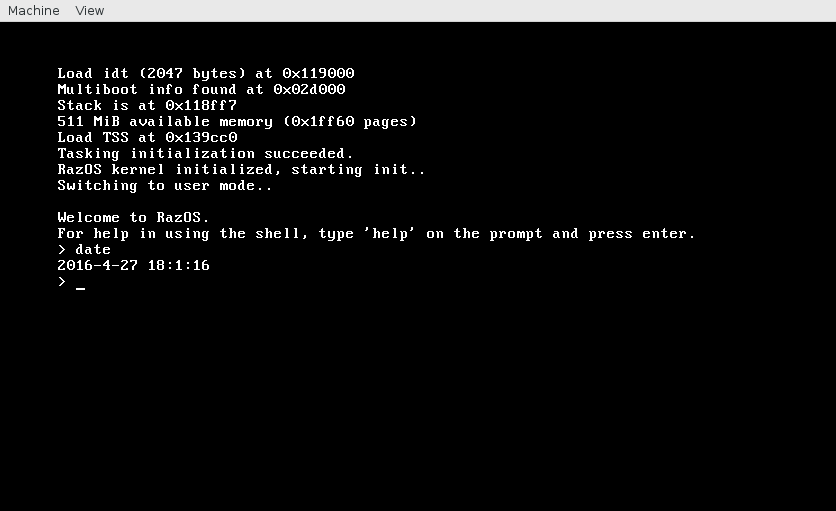
\includegraphics[]{../figures/rash.png}
\label{fig:rash.png}
\end{figure}

\section{Standardityökalut (stdlib.h)}

C-kirjasto stdlib.h määrittelee erilaisia yleishyödyllisiä funktioita, tyyppejä ja makroja, tärkeimpinä dynaamiseen muistinvaraukseen käytettävä malloc, ympäristömuuttujan hallitsemiseen käytettävät getenv- ja setenv-funktiot sekä satunnaislukujen luomiseen käytettävä rand-funktio.

\subsection{Dynaaminen muistinvaraus (malloc)}

Dynaaminen muistinvaraus toimii RazOS:issa hyvin samalla tavoin niin ytimessä kuin käyttäjätilassakin. Käyttäjätilassa jokaisella ohjelmalla on kuitenkin oma virtuaalimuistiavaruus, jossa muistia hallitaan. Koska käyttäjätilalla ei myöskään ole oikeutta käyttää järjestelmäresursseja suoraan, varataan varsinaiset muistisivut brk- ja sbrk-järjestelmäkutsujen avulla.

\subsection{Ympäristömuuttuja (environ)}

Ympäristömuuttuja (environment variable, environ) on osoitin, joka osoittaa merkkijonoista muodostuvaan vektoriin. Nämä merkkijonot sisältävät tietoa ohjelman ympäristöstä, kuten esimerkiksi käytössä olevasta komentotulkista. Kun prosessi kopioidaan fork-järjestelmäkutsulla tai ohjelma aloitetaan exec-järjestelmäkutsulla, ympäristömuuttujan arvot säilyvät.

\par

Koska environ-muuttujan merkkijonojen manuaalinen muuttaminen on virhealtista, POSIX-standardiin kuuluu sen muuttamiseen ja noutamiseen käytettävät setenv- ja getenv-funktiot. Ne on toteutettu myös RazOS:issa.

\subsection{Satunnaisluvut (rand)}

C-kirjaston rand-funktio on näennäissatunnaislukugeneraattori, joka pyrkii matemaattisilla operaatioilla luomaan annetusta siemenarvosta mahdollisimman satunnaisen luvun. RazOS:in rand-funktio täyttää yksinkertaisuudestaan huolimatta C99-standardin minimivaatimukset, ja perustuukin standardin ehdotukseen.

\begin{footnotesize}
\begin{minted}[linenos]{C}
#include <stdlib.h>

static unsigned long next = 1; /* For the rand implementation. */

int rand(void)
{
	next = next * 1103515245 + 12345;
	return((unsigned)(next/65536) % 32768);
}

void srand(unsigned int seed)
{
	next = seed;
}
\end{minted}
\end{footnotesize}

\section{Syöte ja tulostus (stdio.h)}

Tärkeimmät syötteeseen ja tulostukseen liittyvät funktiot löytyvät C-kirjastossa stdio-ylätunnisteen alta. Kirjaston toiminta perustuu täysin käyttöjärjestelmäytimen read- ja write-järjestelmäkutsuihin, sillä vain ydin voi hallita tietokoneen laitteistoja, kuten näyttöä ja näppäimistöä. Käyttäjätilan ohjelmat lukevat ja tulostavat muiden mekanismien avulla, joita Unixissa ovat tekstivirrat ja tiedostodeskriptorit. Jokaiseen tiedostodeskriptoriin liittyy tekstivirta, ja toisaalta jokaista tekstivirtaa vastaa tiedostodeskriptori. Myös standardisyöte (stdin) ja -tuloste (stdout) ovat tiedostodeskriptoreja, joten niitä voidaan käsitellä kuten muitakin tiedostoja. Järjestelmän käsittäminen tiedostojen avulla onkin yksi Unixin periaatteellisista kulmakivistä.

\par

Toinen tärkeä osa Unixin syöte- ja tulostustoimintoja on tekstivirtojen uudelleenohjaus (redirection): ohjelman tuloste voidaankin ohjata johonkin tiedostoon tai toisen ohjelman syötteeksi. Samaten syöte voi tulla näppäimistöltä, toiselta ohjelmalta tai tiedostosta. Ohjelman itse ei tarvitse kuin lukea stdin-tiedostodeskriptoria, sillä järjestelmä hoitaa tekstivirtojen uudelleenohjauksen. Tämä monipuolisuus on syy siihen, miksi Unix käyttää tekstivirtoja yleisenä rajapintana ohjelmien, tiedostojen ja käyttäjien välillä.

\par

RazOS ei syöte- tai tulostustoiminnoiltaan eroa muista POSIX-yhteensopivista Unix-käyttöjärjestelmistä. Käytännön tasolla tekstivirtojen uudelleenohjaus toteutetaan pipe-järjestelmäkutsulla, ja tiedostodeskriptorien luonti vastaavasti dup- ja dup2-järjestelmäkutsuilla. Itse stdio-kirjasto vastaa myös toteutetuilta osin POSIX-standardia, sisältäen esimerkiksi printf-funktion eri muunnelmat.

\section{Komentotulkki}

Komentotulkki on yksi tärkeimmistä ohjelmista Unix-käyttöjärjestelmässä. Se vastaa ohjelmien käynnistämisestä ja prosessinhallinnasta, tekstivirtojen uudelleenohjaamisesta sekä automaatiosta. RazOS:in komentotulkki, Rash, tukee Shell-ohjelmointia lukuun ottamatta näitä komentotulkin perustoimintoja. Erikoisasemastaan huolimatta komentotulkki on Unixissa, kuten RazOS:issakin, vain ohjelma muiden joukossa, eikä sen tiiviimpi osa käyttöjärjestelmää kuin mikään muukaan ohjelma.

\par

Korkealla tasolla komentotulkin toimintaperiaate on varsin yksinkertainen, josta osoituksena alla oleva Rashin syöte-tuloste -silmukka:

\begin{footnotesize}
\begin{minted}[linenos]{C}
static void rash_loop(void)
{
    char *line;
    char **args;
    int status;
    int args_len;
    int i;

    do
    {
        printf("> ");
        line = rash_read_line();
        args = rash_split_line(line, &args_len);
        status = rash_execute(args);

        free(line);
        for (i = 0; i < args_len; i++)
            free(args[i]);
        free(args);
    } while (status);
}
\end{minted}
\end{footnotesize}

Komentotulkin kehitystyö tehtiin GNU/Linux-ympäristössä, josta se siirrettiin pienin muutoksin osaksi RazOS:ia.

\section{Esimerkki standardinmukaisuudesta}

Alla on pieni C-ohjelma, joka tulostaa näytölle päivämäärän ja kellonajan.

\begin{footnotesize}
\begin{minted}[linenos]{C}
#include <stdio.h>
#include <time.h>

int main(void)
{
	time_t t = time(NULL);
	struct tm tm_now = *gmtime(&t);

	printf("%d-%d-%d %d:%d:%d\n",
			tm_now.tm_year + 1900,
			tm_now.tm_mon + 1,
			tm_now.tm_mday,
			tm_now.tm_hour,
			tm_now.tm_min,
			tm_now.tm_sec);
	return 0;
}
\end{minted}
\end{footnotesize}

Ohjelma toimii ilman muutoksia niin RazOS:issa, muissa Unixeissa kuin kaikissa C99-standardin ohjelmointikirjastot sisältävissä käyttöjärjestelmissä.
